\documentclass[twocolumn]{article}
\author{}
\usepackage{graphicx} %I need to include some graphs in this document
\usepackage{amsmath}
\usepackage{caption}
\usepackage{subcaption}
%\usepackage[margin=1.4in]{geometry}
\begin{document}
%\date{} %remove the date after the title
\setcounter{section}{2}
\begin{center}
\section{TEST}
\end{center}
%\setcounter{equation}{9}
\subsection*{COMPUTATION DETAILS}
\paragraph*{}
So far, we have tested this algorithm on liquid and it may be interesting to try it on crystal. Although the Fourier component of $\kappa$ remains constant until q is very large, this is not the case for crystal. One of the simplest model may be the LJ crystal with $fcc$ structure and we based our test on parameters from real crystal of Argon, so we can compare simulations with results from experiments.
\paragraph*{}
We choose the crystal constant as $a=5.31\AA$ which is $a^*=1.56$ in LJ reduced unit (with LJ coefficient $\sigma$ of Argon 3.4 $\AA$).The simulations are conducted on supoercells of $6\times6\times{N}$ cubic conventional cells with $N$ a parameter for approching the bulk limit. This 6 by 6 simulation proves reasonable from comparing the behaviour of $\kappa(q)$ around the $q=0$ with that predicted by Debye Model and in order to do this, we treated the solution of Boltzmann equation in two different ways.
\end{document}
\paragraph*{}
So the Debye prediction gives a thermal conductivty $\kappa_D=3nk_Bv\Lambda_{min}/(3-p)$. With $kappa_D$ as a scaling factor, we can get the general picture of how Fourier component of $\kappa$ approaches the valuve of thermal conductivity.
Firstly, theory parts goes in the way we do the integration over Debye Sphere, the anwser is
\begin{align}
&\frac{\kappa(q)}{\kappa_D}=\frac{3(3-p)\cos^2(qd/2)}{2\omega_D^3}\cdot\nonumber\\
&\int\limits_0^{\omega_D} d\omega\omega^2\int\limits_0^{\pi}d\theta{\sin\theta}{\cos^2\theta}\left(\frac{\omega_D}{\omega}\right)^pF(q,\Lambda_{Qx})\\
&=\frac{3(3-p)}{2}\cos^2(\frac{qd}{2})\int\limits_0^1 dxx^{2-p}\int\limits_0^{\pi}d\theta \sin{\theta}\cos^2{\theta}F(q,\Lambda_{Qx})%\frac{\Lambda_{min}\left(\frac{\omega_D}{\omega}\right)^p\cos{\theta}}{d}
\end{align}
with
\begin{equation}
F(q,\Lambda)=\left\{1+4\sin^2\left(\frac{qd}{2}\right)\left[\left\frac{\Lambda}{d}+\left(\frac{\Lambda}{d}\right)^2\right]\right\}^{-1}
\end{equation}
Here
It is easy to get the $\kappa(q)$ using numerical integral, which is shown in figure below.%!!!cite figure here

\begin{figure}
\begin{subfigure}[htb!]{.5\linewidth}
    \centering
    \caption{The curve of $\kappa(q)$ from integrating in Debye Sphere}
    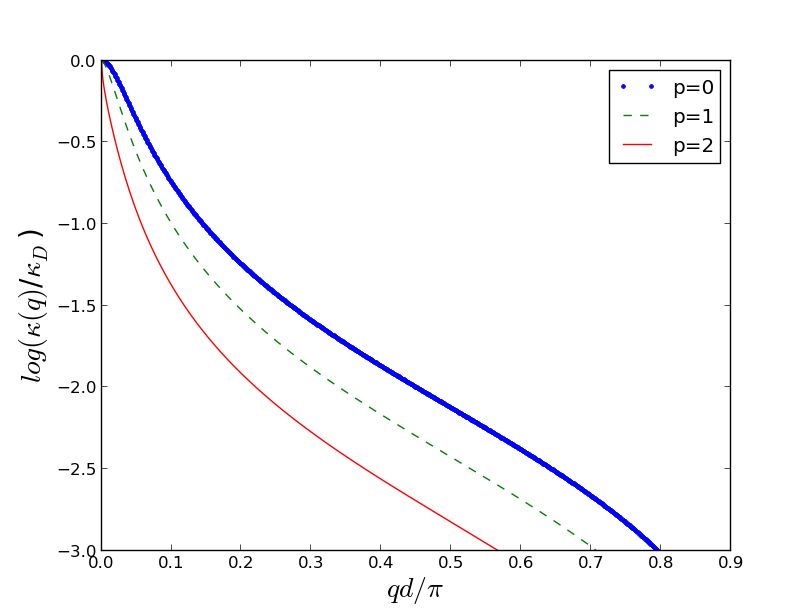
\includegraphics[height=3cm]{DebyeIn.png}
%    %\label{fig:a}
\end{subfigure}
\begin{subfigure}[htb!]{.5\linewidth}
    \centering
    \caption{The curve of $\kappa(q)$ from summing all the points in the Brillouin Zone of the simulation supercell}
    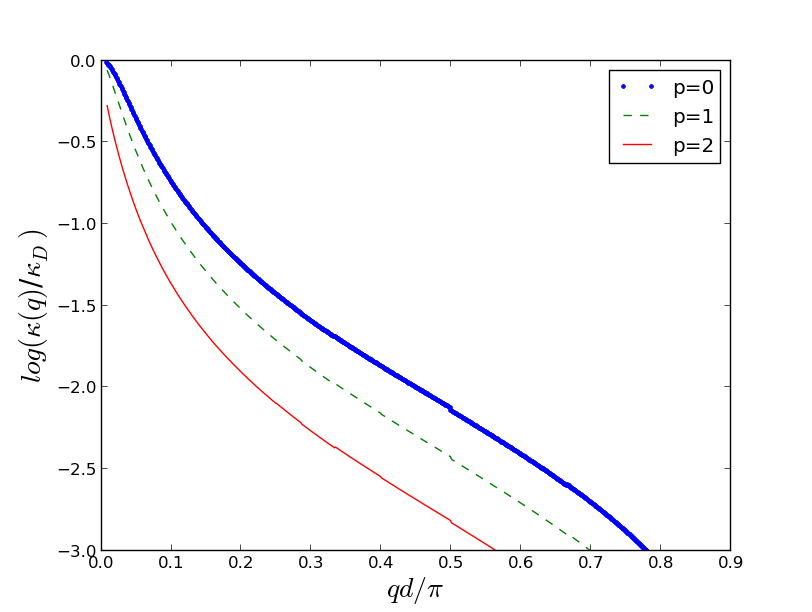
\includegraphics[height=3cm]{BZ.png}
%    %\label{fig:a}
\end{subfigure}
\end{figure}
\paragraph*{}
%To see whether our $6\times 6\times N$ supercells work well, we can try summing up all the wavevector in Brillizone. Although it is useful to have a simplified standard model to replace the Brillouin Zone with Debye Sphere of radius $Q_D$, doing this calculation over points in the true Brillouin Zone can give us a more precise picture of the deviation caused by simulations on crystals which possess Brillouin Zones dense enough merely in one direction.    
\paragraph*{}
%Figure 1 (b) shows how the Fourier component of $\kappa$ behaves on the Brillouzon and we can see it resembles the calculations in Debye sphere.
\paragraph*{}
%A further evaluation on the six by six cell model can tell us that for q's which are small enough, $\kappa(q)$'s hardly have any dependence on q's at all. And actually the variance of $kappa(q)$ for different cross sections appear small.
\begin{figure}
\begin{subfigure}[htb!]{.5\linewidth}
    \centering
    \caption{The curve of $\kappa(q)$ from integrating in Debye Sphere}
    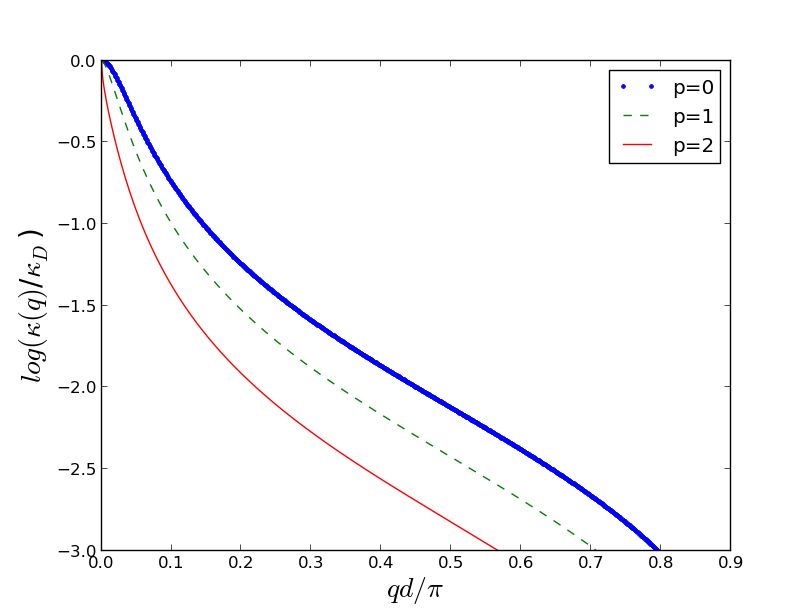
\includegraphics[height=3cm]{DebyeIn.png}
%    %\label{fig:a}
\end{subfigure}
\begin{subfigure}[htb!]{.5\linewidth}
    \centering
    \caption{The curve of $\kappa(q)$ from integrating in Debye Sphere}
    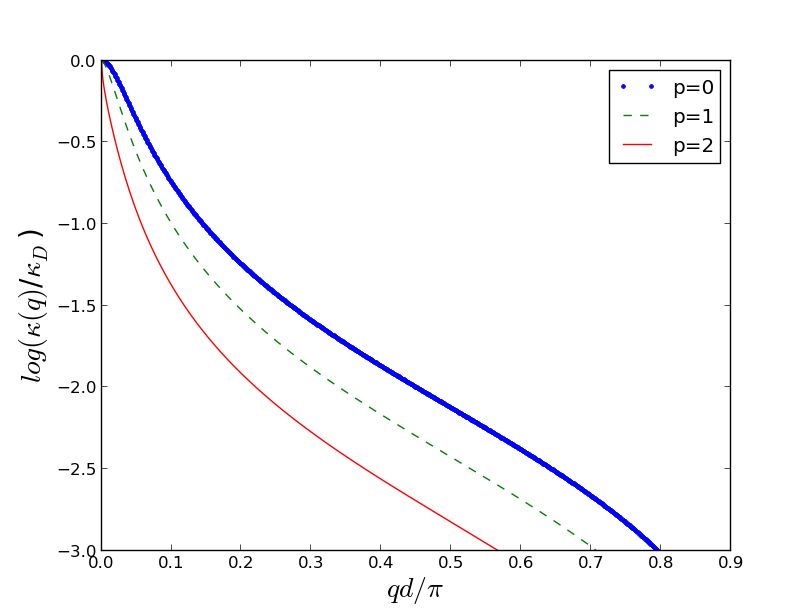
\includegraphics[height=3cm]{DebyeIn.png}
%    %\label{fig:a}
\end{subfigure}
\end{figure}
\begin{table}
\begin{tabular}{p{1.6cm}|p{1.7cm} p{1.7cm} p{1.7cm}}
\hline
\hline
{$\dot{e}$}&{$\kappa(\sigma_\kappa)$ }&{$\sigma_\kappa/\kappa$}&{Stimulation Steps}\\
\hline
0.633                              &   7.25(0.24)   & 3.26\%         & 576210\\
1.265                              &   7.12(0.12)   & 1.69\%         & 96000\\
1.265                              &   7.00(0.07)   & 1.03\%         & 192010\\
2.530                              &   6.81(0.08)   & 1.17\%         & 96000\\
5.060                              &   7.12(0.05)   & 0.70\%        & 24000\\
\hline
Experiment                         &   7.02\footnote{Experiment data for Argon    Handbook of Chemistry and Physics, 74th ed., edited by D. R. Lide Chemical Rubber, Boca Raton, 1993} \\
\hline
\end{tabular}
\end{table}
\paragraph*{}
Table 1 presents the simulation results on crystal 

